\subsection{Plain objects}
\label{subsec:library_of_transformations:instance_level_transformations:plain_objects}

\begin{figure}[b]
    \centering
    \begin{subfigure}{0.45\textwidth}
        \centering
        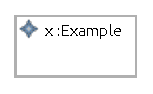
\includegraphics{images/05_library_of_transformations/03_instance_level_transformations/01_plain_objects/class_instance.pdf}
        \caption{$Im_{Class}$ with one object identified as $x$}
        \label{fig:library_of_transformations:instance_level_transformations:plain_objects:visualisation:ecore}
    \end{subfigure}
    \begin{subfigure}{0.45\textwidth}
        \centering
        % To use this figure in your LaTeX document
% import the package groove/resources/groove2tikz.sty
%
\begin{tikzpicture}[scale=\tikzscale,name prefix=start-]
\node[basic_node] (n0) at (1.620, -0.370) {\ml{\uline{\textit{x}} : \textbf{Example}}};

\end{tikzpicture}

        \caption{$IG_{Class}$ with one node identified as $x$}
        \label{fig:library_of_transformations:instance_level_transformations:plain_objects:visualisation:groove}
    \end{subfigure}
    \caption{Visualisation of the transformation of plain objects typed by regular classes}
    \label{fig:library_of_transformations:instance_level_transformations:plain_objects:visualisation}
\end{figure}

The first transformation that will be defined is a transformation of plain objects of a regular class type. The corresponding type level transformation can be found in \cref{subsec:library_of_transformations:type_level_transformations:regular_classes}. This transformation introduces an arbitrary amount of instances of the class introduced on the type level. First, the definition of the corresponding instance model is given.

\begin{defin}[Instance model $Im_{Class}$]
\label{defin:library_of_transformations:instance_level_transformations:plain_objects:imod_class}
Let $Im_{Class}$ be the instance model containing a set of objects $objects$ which are all typed by class $name$. Furthermore, an injective function $fid$ is defined which maps every object in the set to its corresponding identifier. $Im_{Class}$ is typed by $Tm_{Class}$ (\cref{defin:library_of_transformations:type_level_transformations:regular_classes:tmod_class}) and is defined as:
\begin{align*}
Object =\ &objects \\
\mathrm{ObjectClass} =\ & \begin{cases}
    (ob, name) & \mathrm{if }\ ob \in objects
\end{cases}\\
\mathrm{ObjectId} =\ & \begin{cases}
    (ob, fid(ob)) & \mathrm{if }\ ob \in objects
\end{cases}\\
\mathrm{FieldValue} =\ & \{\} \\
\mathrm{DefaultValue} =\ & \{\}
\end{align*}
\isabellelref{imod_class}{Ecore-GROOVE-Mapping-Library.ClassInstance}
\end{defin}

\begin{thm}[Correctness of $Im_{Class}$]
\label{defin:library_of_transformations:instance_level_transformations:plain_objects:imod_class_correct}
$Im_{Class}$ (\cref{defin:library_of_transformations:instance_level_transformations:plain_objects:imod_class}) is a valid instance model in the sense of \cref{defin:formalisations:ecore_formalisation:instance_models:model_validity}.
\isabellelref{imod_class_correct}{Ecore-GROOVE-Mapping-Library.ClassInstance}
\end{thm}

A visual representation of $Im_{Class}$ with $objects = \{ob\}$ and $fid(ob) = x$ can be seen in \cref{fig:library_of_transformations:instance_level_transformations:plain_objects:visualisation:ecore}. Although this visualisation only shows one object, it is possible to have an arbitrary amount of objects in $Im_{Class}$, as long as they are all typed by the corresponding class introduced on the type level. In the visualisation, the identifier $.\type{Example}$ is used for the class, in correspondence with \cref{fig:library_of_transformations:type_level_transformations:regular_classes:visualisation:ecore} The correctness proof of $Im_{Class}$ is trivial, and therefore not included here. The proof can be found as part of the Isabelle validated proofs.

In order to make composing transformation functions possible, $Im_{Class}$ should be compatible with the instance model it is combined with.

\begin{thm}[Correctness of $\mathrm{combine}(Im, Im_{Class})$]
\label{defin:library_of_transformations:instance_level_transformations:plain_objects:imod_class_combine_correct}
Assume an instance model $Im$ that is valid in the sense of \cref{defin:formalisations:ecore_formalisation:instance_models:model_validity}. Then $Im$ is compatible with $Im_{Class}$ (in the sense of \cref{defin:transformation_framework:instance_models_and_instance_graphs:combining_instance_models:compatibility}) if:
\begin{itemize}
    \item All requirements of \cref{defin:library_of_transformations:type_level_transformations:regular_classes:tmod_class_combine_correct} are met, to ensure the combination of the corresponding type models is valid;
    \item All the objects in $Im_{Class}$ have an (internal and explicit) identity that is not yet used in $Im$.
\end{itemize}
\isabellelref{imod_class_combine_correct}{Ecore-GROOVE-Mapping-Library.ClassInstance}
\end{thm}

\begin{proof}
Use \cref{defin:transformation_framework:instance_models_and_instance_graphs:combining_instance_models:imod_combine_merge_correct}. It is possible to show that all assumptions hold. Now we have shown that $\mathrm{combine}(Im, Im_{Class})$ is consistent in the sense of \cref{defin:formalisations:ecore_formalisation:instance_models:model_validity}.
\end{proof}

Please note that this combination is quite trivial, as the newly introduced objects cannot have fields. This is because they are all typed by the new class type introduced in $Tm_{Class}$. Since this new class type is new by assumption, the existing model cannot have fields defined for the class type.

The definitions and theorems for introducing plain objects of regular classes within Ecore are now complete. 

\subsubsection{Encoding as nodes}

A possible encoding for plain objects in Ecore is using nodes in GROOVE. Each node is typed by the node type that was introduced in $TG_{Class}$, and copies the identifiers set of the objects to the corresponding nodes. The encoding corresponding to $Im_{Class}$ can then be represented as $IG_{Class}$, defined in the following definition:

\begin{defin}[Instance graph $IG_{Class}$]
\label{defin:library_of_transformations:instance_level_transformations:plain_objects:ig_class_as_node_type}
Let $IG_{Class}$ be the instance graph with as nodes the converted $objects$ of $Im_{Class}$ (\cref{defin:library_of_transformations:instance_level_transformations:plain_objects:imod_class}). Furthermore, reuse the injective function $fid$ that maps every object to its identifier. Finally, use the node type introduced in $TG_{Class}$ (\cref{defin:library_of_transformations:type_level_transformations:regular_classes:tg_class_as_node_type}). $IG_{Class}$ is defined typed by $TG_{Class}$ and is defined as:
\begin{align*}
N =\ & objects \\
E =\ & \{\} \\
\mathrm{ident} =\ & \begin{cases}
    (fid(ob), ob) & \mathrm{if }\ ob \in objects
\end{cases}
\end{align*}
with
\begin{align*}
\mathrm{type}_n =\ & \begin{cases}
    (ob, \mathrm{ns\_\!to\_\!list}(name)) & \mathrm{if }\ ob \in objects
\end{cases}
\end{align*}
\isabellelref{ig_class_as_node_type}{Ecore-GROOVE-Mapping-Library.ClassInstance}
\end{defin}

\begin{thm}[Correctness of $IG_{Class}$]
\label{defin:library_of_transformations:instance_level_transformations:plain_objects:ig_class_as_node_type_correct}
$IG_{Class}$ (\cref{defin:library_of_transformations:instance_level_transformations:plain_objects:ig_class_as_node_type}) is a valid instance graph in the sense of \cref{defin:formalisations:groove_formalisation:instance_graphs:instance_graph_validity}.
\isabellelref{ig_class_as_node_type_correct}{Ecore-GROOVE-Mapping-Library.ClassInstance}
\end{thm}

A visual representation of $IG_{Class}$ with $objects = \{ob\}$ and $fid(ob) = x$ can be seen in \cref{fig:library_of_transformations:instance_level_transformations:plain_objects:visualisation:groove}. Like the previous example for the Ecore instance model, only one node is shown here, but multiple nodes can be introduced at once if there are more objects in the $objects$ set. As shown in the definition, the node type identified by $\type{Example}$ is used to type all the nodes, in correspondence with \cref{fig:library_of_transformations:type_level_transformations:regular_classes:visualisation:groove}. The correctness proof of $IG_{Class}$ is trivial, and therefore not included here. The proof can be found as part of the Isabelle validated proofs.

In order to make composing transformation functions possible, $IG_{Class}$ should be compatible with the instance graph it is combined with.

\begin{thm}[Correctness of $\mathrm{combine}(IG, IG_{Class})$]
\label{defin:library_of_transformations:instance_level_transformations:plain_objects:ig_class_as_node_type_combine_correct}
Assume an instance graph $IG$ that is valid in the sense of \cref{defin:formalisations:groove_formalisation:instance_graphs:instance_graph_validity}. Then $IG$ is compatible with $IG_{Class}$ (in the sense of \cref{defin:transformation_framework:instance_models_and_instance_graphs:combining_instance_graphs:compatibility}) if:
\begin{itemize}
    \item All requirements of \cref{defin:library_of_transformations:type_level_transformations:regular_classes:tg_class_as_node_type_combine_correct} are met, to ensure the combination of the corresponding type graphs is valid;
    \item All the nodes in $IG_{Class}$ have an (internal and explicit) identity that is not yet used in $IG$.
\end{itemize}
\isabellelref{ig_class_as_node_type_combine_correct}{Ecore-GROOVE-Mapping-Library.ClassInstance}
\end{thm}

\begin{proof}
Use \cref{defin:transformation_framework:instance_models_and_instance_graphs:combining_instance_graphs:ig_combine_merge_correct}. It is possible to show that all assumptions hold. Now we have shown that $\mathrm{combine}(IG, IG_{Class})$ is valid in the sense of \cref{defin:formalisations:groove_formalisation:instance_graphs:instance_graph_validity}.
\end{proof}

The next definitions define the transformation function from $Im_{Class}$ to $IG_{Class}$:

\begin{defin}[Transformation function $f_{Class}$]
\label{defin:library_of_transformations:instance_level_transformations:plain_objects:imod_class_to_ig_class_as_node_type}
The transformation function $f_{Class}(Im)$ is defined as:
\begin{align*}
N =\ & Object_{Im} \\
E =\ & \{\} \\
\mathrm{ident} =\ & \begin{cases}
    (fid(ob), ob) & \mathrm{if }\ ob \in Object_{Im}
\end{cases}
\end{align*}
with
\begin{align*}
\mathrm{type}_n =\ & \begin{cases}
    (ob, \mathrm{ns\_\!to\_\!list}(name)) & \mathrm{if }\ ob \in Object_{Im}
\end{cases}
\end{align*}
\isabellelref{imod_class_to_ig_class_as_node_type}{Ecore-GROOVE-Mapping-Library.ClassInstance}
\end{defin}

\begin{thm}[Correctness of $f_{Class}$]
\label{defin:library_of_transformations:instance_level_transformations:plain_objects:imod_class_to_ig_class_as_node_type_func}
$f_{Class}(Im)$ (\cref{defin:library_of_transformations:instance_level_transformations:plain_objects:imod_class_to_ig_class_as_node_type}) is a valid transformation function in the sense of \cref{defin:transformation_framework:instance_models_and_instance_graphs:combining_transformation_functions:transformation_function_instance_model_instance_graph} transforming $Im_{Class}$ into $IG_{Class}$.
\isabellelref{imod_class_to_ig_class_as_node_type_func}{Ecore-GROOVE-Mapping-Library.ClassInstance}
\end{thm}

The proof of the correctness of $f_{Class}$ will not be included here. Instead, it can be found in the validated Isabelle theories. The proof is quite trivial, as extending $Im$ can only add extra objects, but not remove the existing ones.

Finally, to complete the transformation, the transformation function that transforms $IG_{Class}$ into $Im_{Class}$ is defined:

\begin{defin}[Transformation function $f'_{Class}$]
\label{defin:library_of_transformations:instance_level_transformations:plain_objects:ig_class_as_node_type_to_imod_class}
The transformation function $f'_{Class}(IG)$ is defined as:
\begin{align*}
Object =\ &N_{IG} \\
\mathrm{ObjectClass} =\ & \begin{cases}
    (ob, name) & \mathrm{if }\ ob \in N_{IG}
\end{cases}\\
\mathrm{ObjectId} =\ & \begin{cases}
    (ob, fid(ob)) & \mathrm{if }\ ob \in N_{IG}
\end{cases}\\
\mathrm{FieldValue} =\ & \{\} \\
\mathrm{DefaultValue} =\ & \{\}
\end{align*}
\isabellelref{ig_class_as_node_type_to_imod_class}{Ecore-GROOVE-Mapping-Library.ClassInstance}
\end{defin}

\begin{thm}[Correctness of $f'_{Class}$]
\label{defin:library_of_transformations:instance_level_transformations:plain_objects:ig_class_as_node_type_to_tmod_class_func}
$f'_{Class}(IG)$ (\cref{defin:library_of_transformations:instance_level_transformations:plain_objects:ig_class_as_node_type_to_imod_class}) is a valid transformation function in the sense of \cref{defin:transformation_framework:instance_models_and_instance_graphs:combining_transformation_functions:transformation_function_instance_graph_instance_model} transforming $IG_{Class}$ into $Im_{Class}$.
\isabellelref{ig_class_as_node_type_to_imod_class_func}{Ecore-GROOVE-Mapping-Library.ClassInstance}
\end{thm}

Once more, the correctness proof is not included here but can be found in the validated Isabelle proofs of this thesis.